\section{Additional Software Outputs}\label{sec:additional-outputs}


\subsection{Heatmap}

The \texttt{GLaRe()} function also returns a heatmap to display the full distribution of information losses (Figure \ref{fig:eye-heatmap}).
It is obtained by re-ordering the $N$ values within each column of the matrix of cross-validated information losses.
Then the latent feature dimension is represented on the $x$-axis, the corresponding quantile of the column on the $y$-axis and the color represents the information loss.


\begin{figure}
    \centering
    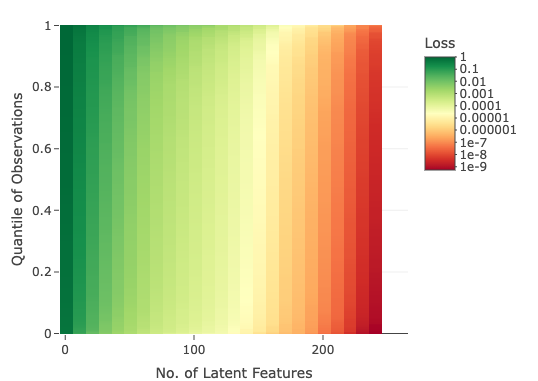
\includegraphics[width=0.75\linewidth]{figures/eye-heatmap.png}
    \caption{{\color{purple}Note: Reverse color ordering.}}
    \label{fig:eye-heatmap}
\end{figure}

\subsection{Additional Summary Plots}

The \pkg{GLaRe} package also contains wrapper functions that plots to summaries the cross-validated distribution of information losses; their outputs are displayed in Figure \ref{fig:additional-plots-01}.
The function \texttt{distribution\_plot()} produces a dot-plot of the individual cross-validated information loss distribution, where each point represents an individual value and the points are colored according to the latent feature dimension $K$ (Figure \ref{fig:additional-plots-01} \textbf{(a)}).

\begin{figure}
    \centering
    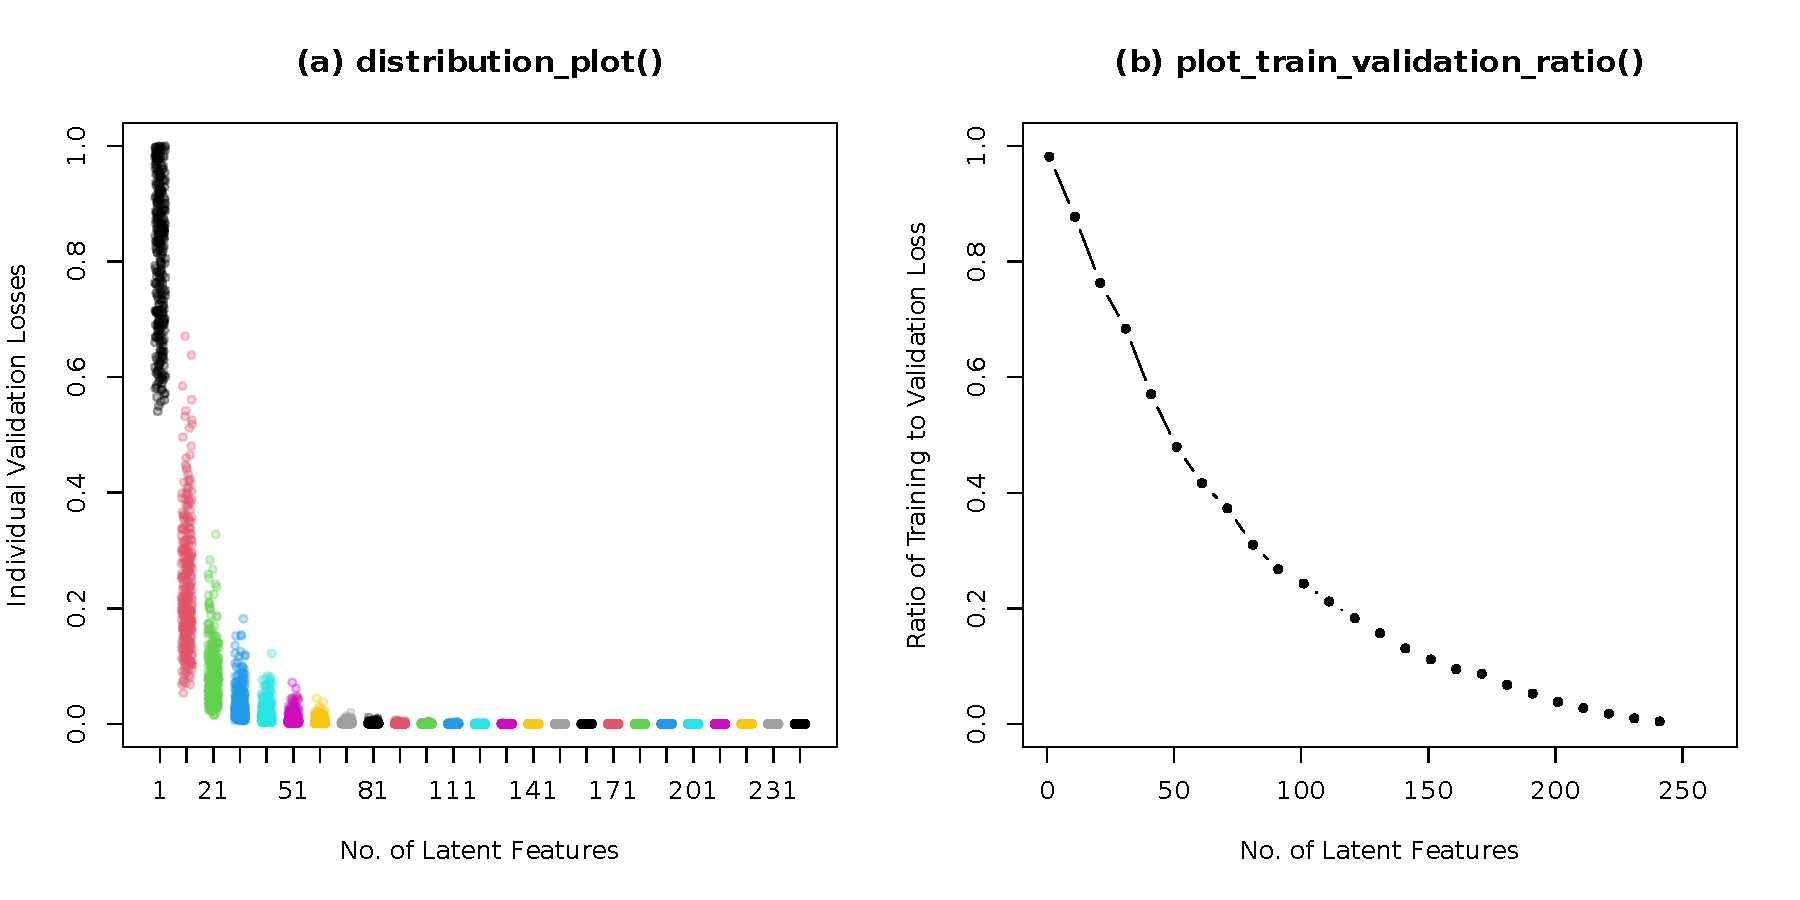
\includegraphics[width=1\linewidth]{figures/additional-plots-01.pdf}
    \caption{Additional wrapper functions that produce summary plots of \texttt{GLaRe()} outputs. \textbf{(a)} \texttt{distribution\_plot()} produces a dot-plot of the individual cross-validated information loss distribution. \textbf{(b)} \texttt{plot\_train\_validation\_ratio()} produces a point and line plot of the ratio of the total training and validation losses.
    Both plots are demonstrated on the Glaucoma dataset with a PCA representation from Section \ref{sec:software}.}
    \label{fig:additional-plots-01}
\end{figure}

\subsection{Reconstruction Plots}

Figure \ref{fig:eye-reconstruction}.

\begin{figure}
    \centering
    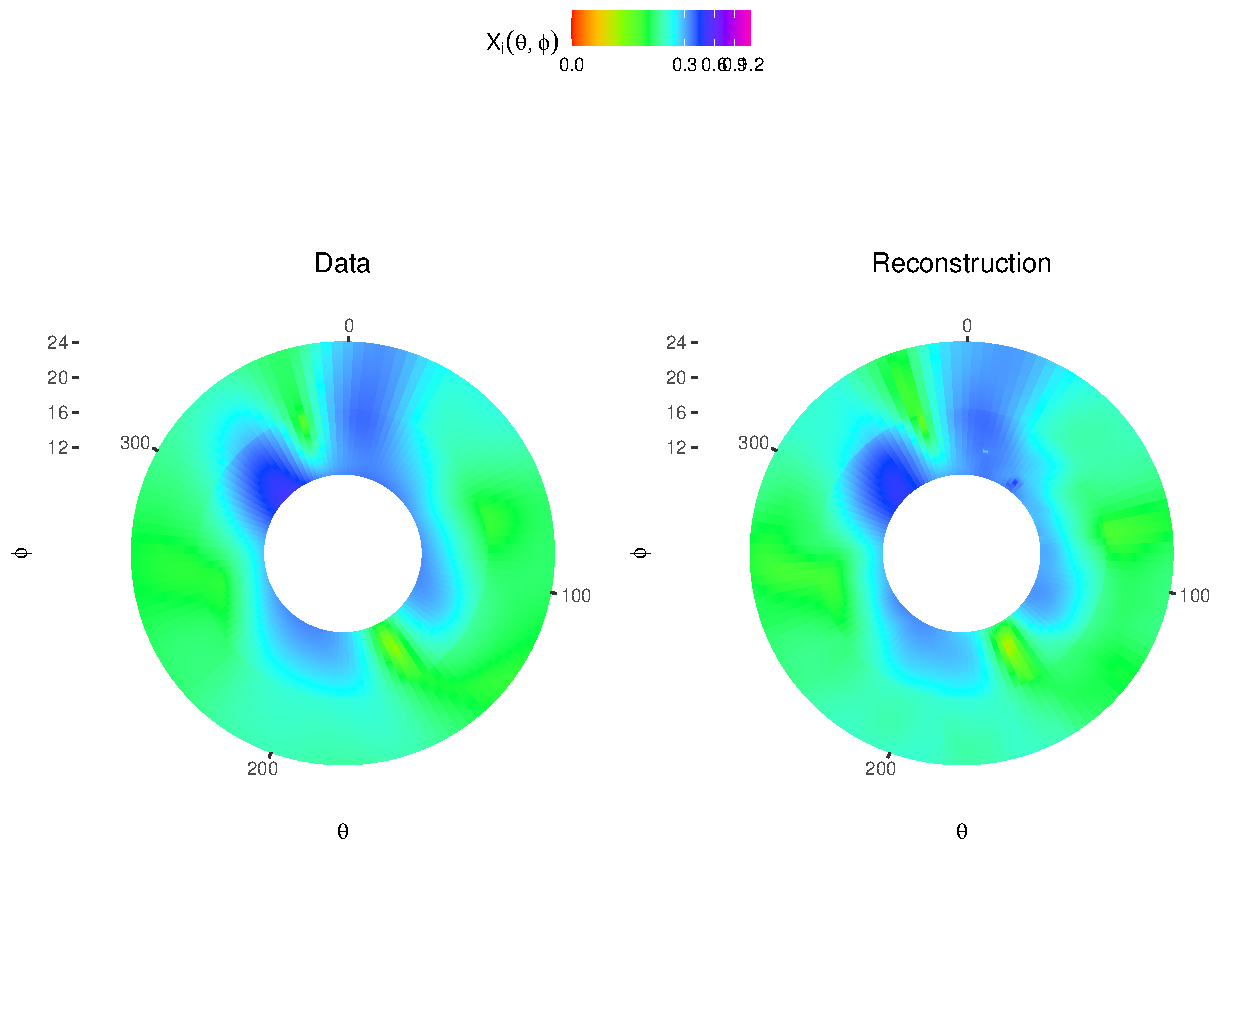
\includegraphics[width=0.75\linewidth]{figures/eye-reconstruction.pdf}
    \caption{Caption\jsm{[BE SURE TO INSERT CAPTION HERE]}}
    \label{fig:eye-reconstruction}
\end{figure}


\begin{figure}
    \centering
    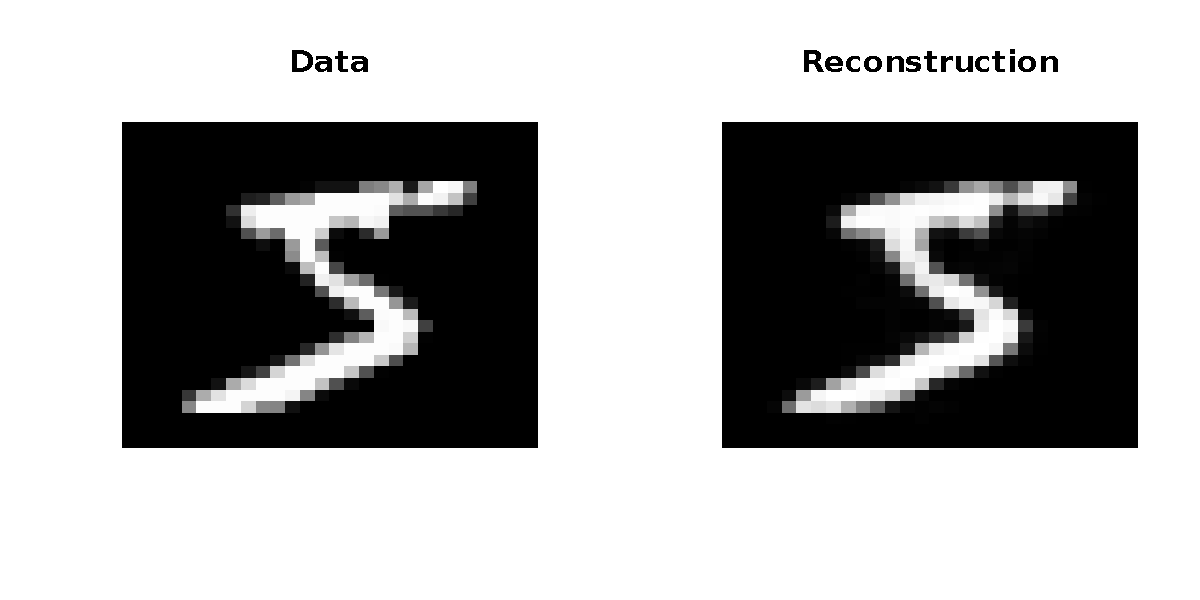
\includegraphics[width=0.75\linewidth]{figures/mnist-reconstruction.pdf}
    \caption{Caption\jsm{[BE SURE TO INSERT CAPTION HERE]}}
    \label{fig:mnist-reconstruction}
\end{figure}